\section{实验要求与实验目的}

\subsection{实验要求}
本实验要求利用 AT89C51 单片机的 T1 计数输入端 P3.5 对外部脉冲进行计数，并通过 LED 数码管动态显示计数结果。脉冲信号可由按钮或外部信号源提供，进入单片机前需要经过两级 74LS14 施密特触发反相器整形，使输入到 T1 端的脉冲边沿更加清晰。

显示部分沿用 P0 口扩展方案：P0.0--P0.7 同时连接两片 SN74HC573 的 D0--D7，一片作为段码锁存器，一片作为位码锁存器；P2.6 控制段码锁存，P2.7 控制位码锁存。控制部分使用 INT0 按钮作为启动/停止键，INT1 按钮作为清零键，两个按键均采用外部中断响应。系统复位后显示 ``000000''，第一次按下 INT0 后开始计数，再按一次停止计数，再按则在原数值基础上继续计数；按下 INT1 后停止计数并清零。

\subsection{实验目的}
\begin{enumerate}
  \item 理解单片机定时/计数器作为外部计数器时的工作原理。
  \item 掌握多字节十进制数的加 1 和进位处理方法。
  \item 掌握外部中断的下降沿触发方式，以及用中断实现按键控制的方法。
  \item 巩固 P0 口经 SN74HC573 扩展后驱动 LED 数码管动态显示的方法。
\end{enumerate}

\subsection{总体设计思路}
系统由脉冲输入整形、外部中断控制、T1 计数和 LED 数码管显示四部分组成。外部脉冲经两级 74LS14 后送入 P3.5/T1，Timer1 设置为方式 2 计数器模式，并把 TH1、TL1 置为 FFH，使每输入一个脉冲即产生一次溢出中断。程序在 Timer1 中断中对六位十进制显示缓冲区加 1，主循环不断扫描显示缓冲区，从而实时显示当前脉冲数。

\begin{figure}[H]
\centering
\resizebox{0.96\textwidth}{!}{%
\begin{tikzpicture}[
  node distance=9mm and 12mm,
  block/.style={rectangle,rounded corners,draw=themecolor,fill=blue!3,minimum width=3.8cm,minimum height=9mm,align=center},
  io/.style={trapezium,trapezium left angle=75,trapezium right angle=105,draw=accentgreen,fill=green!8,minimum width=3.9cm,minimum height=9mm,align=center},
  line/.style={-Latex,thick,draw=themecolor}
]
  \node[io] (pulse) {按钮/外部\\脉冲信号};
  \node[block,right=of pulse] (schmitt) {两级 74LS14\\脉冲整形};
  \node[block,right=of schmitt] (mcu) {AT89C51\\T1计数与中断控制};
  \node[block,right=of mcu,yshift=8mm] (seg) {SN74HC573\\段码锁存};
  \node[block,right=of mcu,yshift=-8mm] (bit) {SN74HC573\\位码锁存};
  \node[io,right=15mm of seg,yshift=-8mm] (led) {LED 数码管\\显示 000000};

  \draw[line] (pulse) -- (schmitt);
  \draw[line] (schmitt) -- node[above,font=\small] {P3.5/T1} (mcu);
  \draw[line] (mcu) -- node[above,font=\small] {P0 段码} (seg);
  \draw[line] (mcu) -- node[below,font=\small] {P0 位码} (bit);
  \draw[line] (seg) -- node[above,font=\small] {A--DP} (led);
  \draw[line] (bit) -- node[below,font=\small] {1--8 位选} (led);
  \node[block,below=12mm of mcu,minimum width=4.6cm] (key) {INT0：启动/停止\\INT1：清零};
  \draw[line] (key) -- (mcu);
\end{tikzpicture}}
\caption{脉冲计数显示系统结构}
\end{figure}

\section{硬件电路设计}

\subsection{单片机最小系统}
AT89C51 采用 +5V 供电，EA 引脚接高电平，XTAL1、XTAL2 外接晶振和两个 30pF 电容构成时钟电路，RST 引脚连接上电复位和按键复位网络。该部分保证单片机能够稳定取指运行，是全部控制逻辑的基础。

\begin{figure}[H]
  \centering
  \begin{subfigure}{0.47\textwidth}
    \centering
    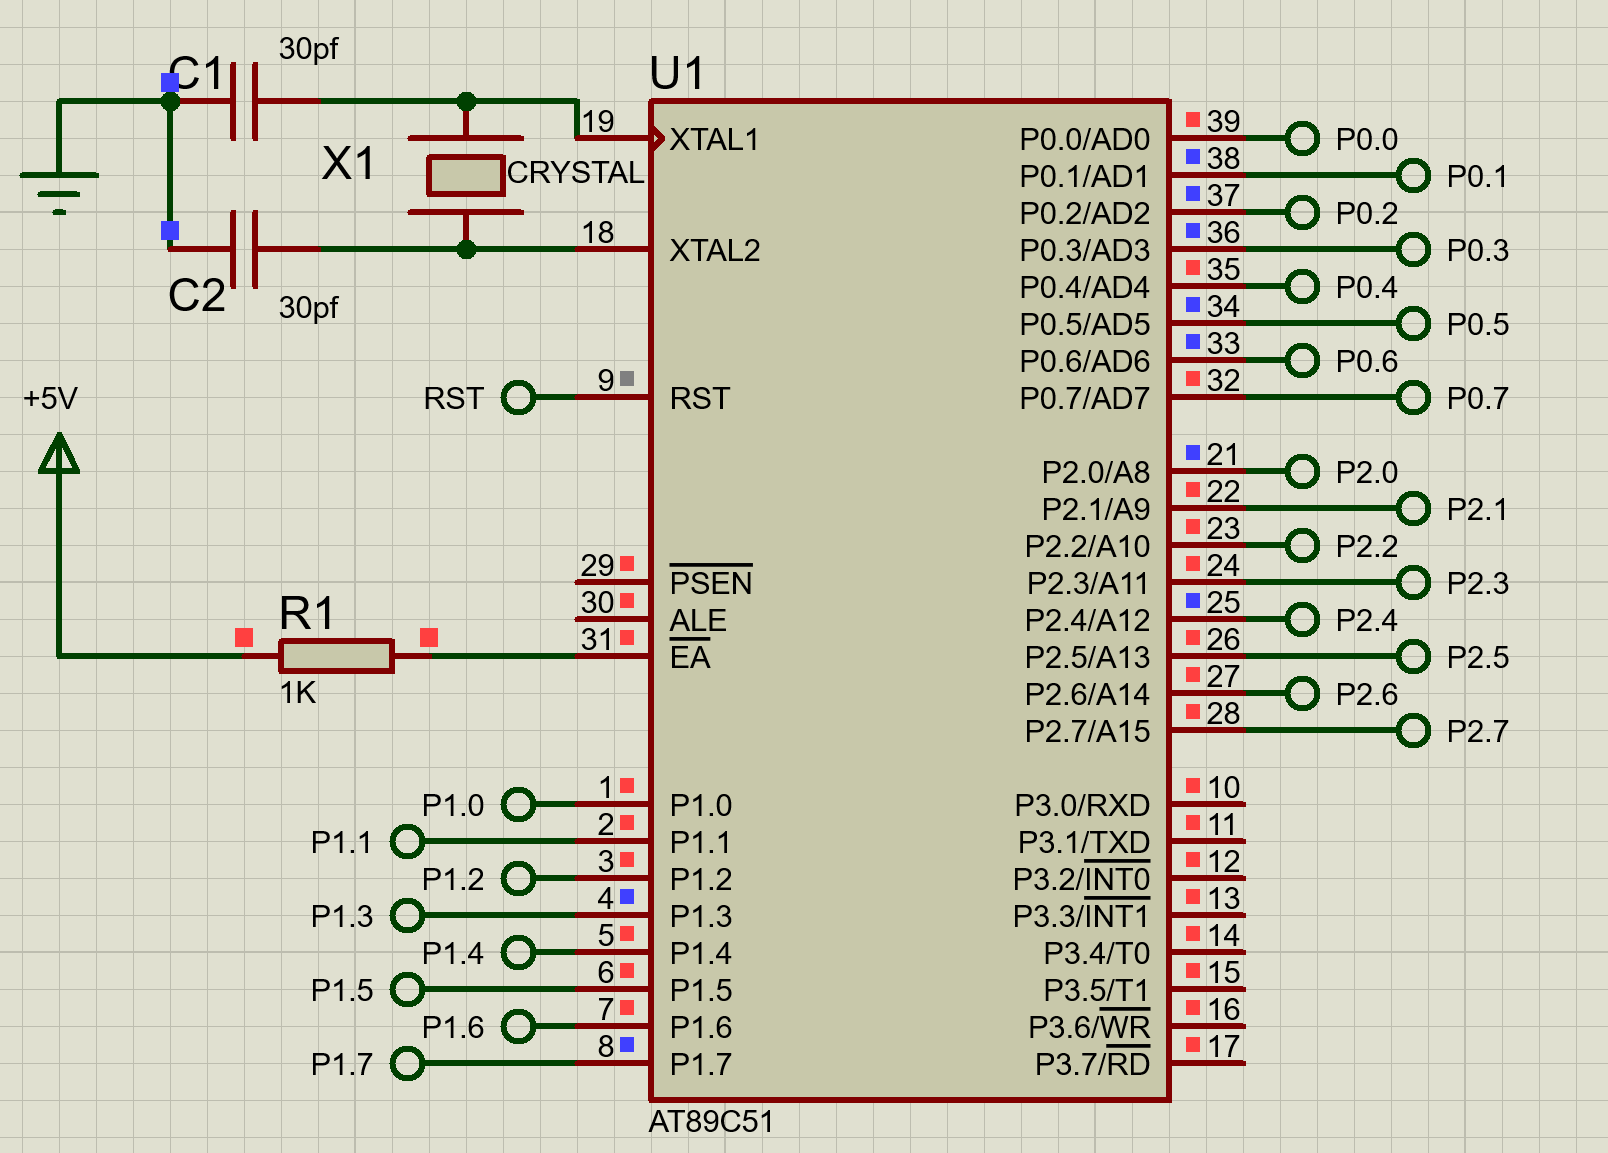
\includegraphics[width=\textwidth]{images/power.png}
    \caption{单片机供电与晶振部分}
  \end{subfigure}
  \hfill
  \begin{subfigure}{0.47\textwidth}
    \centering
    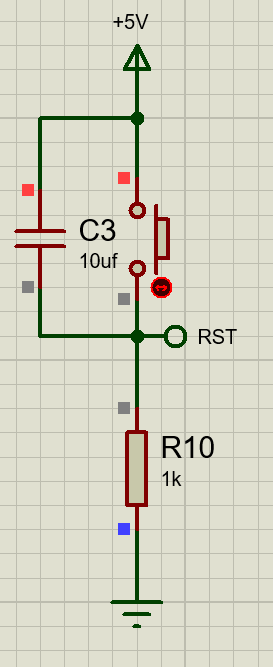
\includegraphics[width=\textwidth]{images/rst.png}
    \caption{复位电路}
  \end{subfigure}
  \caption{单片机基础外围电路}
\end{figure}

\subsection{脉冲输入与 74LS14 整形}
外部脉冲输入端通过上拉电阻保持高电平，按钮按下或外部信号变化时形成脉冲。由于机械按键和外部信号可能存在抖动、边沿缓慢或毛刺，实验中加入两级 74LS14 施密特触发反相器。两级反相后总体逻辑极性保持不变，但波形边沿被整形成更陡峭的数字脉冲，便于 T1 端稳定计数。

\subsection{外部中断按键}
INT0 接 P3.2，用作启动/停止键；INT1 接 P3.3，用作清零键。两个按键均采用上拉电阻接 +5V、按钮接地的方式，未按下时为高电平，按下时产生下降沿。程序中将 IT0、IT1 置 1，使外部中断按下降沿触发，同时把外部中断优先级设置为高，保证按键响应及时。

\subsection{LED 数码管显示电路}
显示电路沿用两片 SN74HC573 扩展 P0 口的结构。段码锁存器的 Q0--Q7 连接数码管 A、B、C、D、E、F、G、DP 段；位码锁存器的 Q0--Q7 连接 8 位数码管的位选端。P2.6 提供段码锁存脉冲，P2.7 提供位码锁存脉冲。程序仅扫描其中 6 位，用于显示从 000000 到 999999 的脉冲计数值。

\begin{table}[H]
  \centering
  \caption{实验五关键端口分配}
  \begin{tabular}{>{\centering\arraybackslash}p{3cm}p{5.2cm}p{5.8cm}}
    \toprule
    单片机端口 & 连接对象 & 功能说明 \\
    \midrule
    P0.0--P0.7 & 两片 SN74HC573 的 D0--D7 & 复用输出段码和位码 \\
    P2.6 & 段码锁存器 LE & 锁存 A--DP 段码 \\
    P2.7 & 位码锁存器 LE & 锁存数码管位选码 \\
    P3.5/T1 & 两级 74LS14 输出 & 外部脉冲计数输入 \\
    P3.2/INT0 & 启动/停止按钮 & 外部中断控制计数启停 \\
    P3.3/INT1 & 清零按钮 & 外部中断清零并停止计数 \\
    \bottomrule
  \end{tabular}
\end{table}

\section{软件设计}

\subsection{程序总体流程}
程序初始化时首先清零 50H--55H 六个显示缓冲单元，使系统复位后显示 ``000000''。随后设置 Timer1 为方式 2 外部计数器模式，设置 INT0、INT1 为下降沿触发，并开启 Timer1 中断、INT0 中断和 INT1 中断。主程序不直接计数，而是循环执行动态显示扫描，计数和按键控制均由中断完成。

\begin{figure}[H]
\centering
\begin{tikzpicture}[
  node distance=8mm,
  proc/.style={rectangle,rounded corners,draw=themecolor,fill=blue!3,minimum width=7.5cm,minimum height=8mm,align=center},
  term/.style={ellipse,draw=accentgreen,fill=green!8,minimum width=4.2cm,minimum height=8mm,align=center},
  line/.style={-Latex,thick,draw=themecolor}
]
  \node[term] (start) {开始};
  \node[proc,below=of start] (init) {初始化显示缓冲区为 000000};
  \node[proc,below=of init] (timer) {Timer1 设为方式2外部计数器};
  \node[proc,below=of timer] (int) {INT0/INT1 设为下降沿触发并开中断};
  \node[proc,below=of int] (disp) {循环动态扫描 LED 数码管};

  \draw[line] (start) -- (init);
  \draw[line] (init) -- (timer);
  \draw[line] (timer) -- (int);
  \draw[line] (int) -- (disp);
  \draw[line] (disp.east) -- ++(1,0) |- (disp.east);
\end{tikzpicture}
\caption{主程序流程图}
\end{figure}

\subsection{中断处理流程}
INT0 中断用于切换运行状态。若当前处于停止状态，按下 INT0 后置位运行标志并启动 TR1；若当前处于运行状态，则清除运行标志并关闭 TR1。INT1 中断用于清零，进入中断后立即关闭 TR1、清除运行标志，并把六位显示缓冲区全部写 0。

Timer1 工作在方式 2 计数器模式时，TH1、TL1 均置为 FFH。外部 T1 输入每来一个脉冲，TL1 从 FFH 溢出并触发 Timer1 中断。中断服务程序重新装入 TL1=FFH，并调用十进制加 1 子程序。加 1 子程序从最低位 55H 开始，如果某一位加到 10，则清零并向高位进位。

\begin{figure}[H]
\centering
\resizebox{0.76\textwidth}{!}{%
\begin{tikzpicture}[
  node distance=6mm,
  proc/.style={rectangle,rounded corners,draw=themecolor,fill=blue!3,minimum width=7.0cm,minimum height=7mm,align=center},
  judge/.style={diamond,aspect=2.2,draw=accentyellow,fill=yellow!10,minimum width=4.0cm,minimum height=8mm,align=center},
  line/.style={-Latex,thick,draw=themecolor}
]
  \node[proc] (t1) {Timer1 溢出中断};
  \node[proc,below=of t1] (reload) {TL1 重新装入 FFH};
  \node[proc,below=of reload] (r0) {R0 指向最低位 55H};
  \node[proc,below=of r0] (inc) {当前十进制位加 1};
  \node[judge,below=of inc] (ten) {是否等于 10};
  \node[proc,below=of ten] (done) {未进位，返回};
  \node[proc,right=18mm of ten] (carry) {本位清 0，向高位进位};

  \draw[line] (t1) -- (reload);
  \draw[line] (reload) -- (r0);
  \draw[line] (r0) -- (inc);
  \draw[line] (inc) -- (ten);
  \draw[line] (ten) -- node[right,font=\small] {否} (done);
  \draw[line] (ten) -- node[above,font=\small] {是} (carry);
  \draw[line] (carry.north) |- (inc.east);
\end{tikzpicture}}
\caption{Timer1 计数中断与十进制进位流程}
\end{figure}

\section{仿真调试与结果}

\subsection{Proteus 仿真电路}
本实验在 Proteus 中完成 AT89C51、两片 SN74HC573、两级 74LS14、按键和 LED 数码管的连接。脉冲输入经 74LS14 整形后进入 T1，INT0 和 INT1 分别用于启停和清零，显示部分在 6 位数码管上输出当前计数值。

\begin{figure}[H]
  \centering
  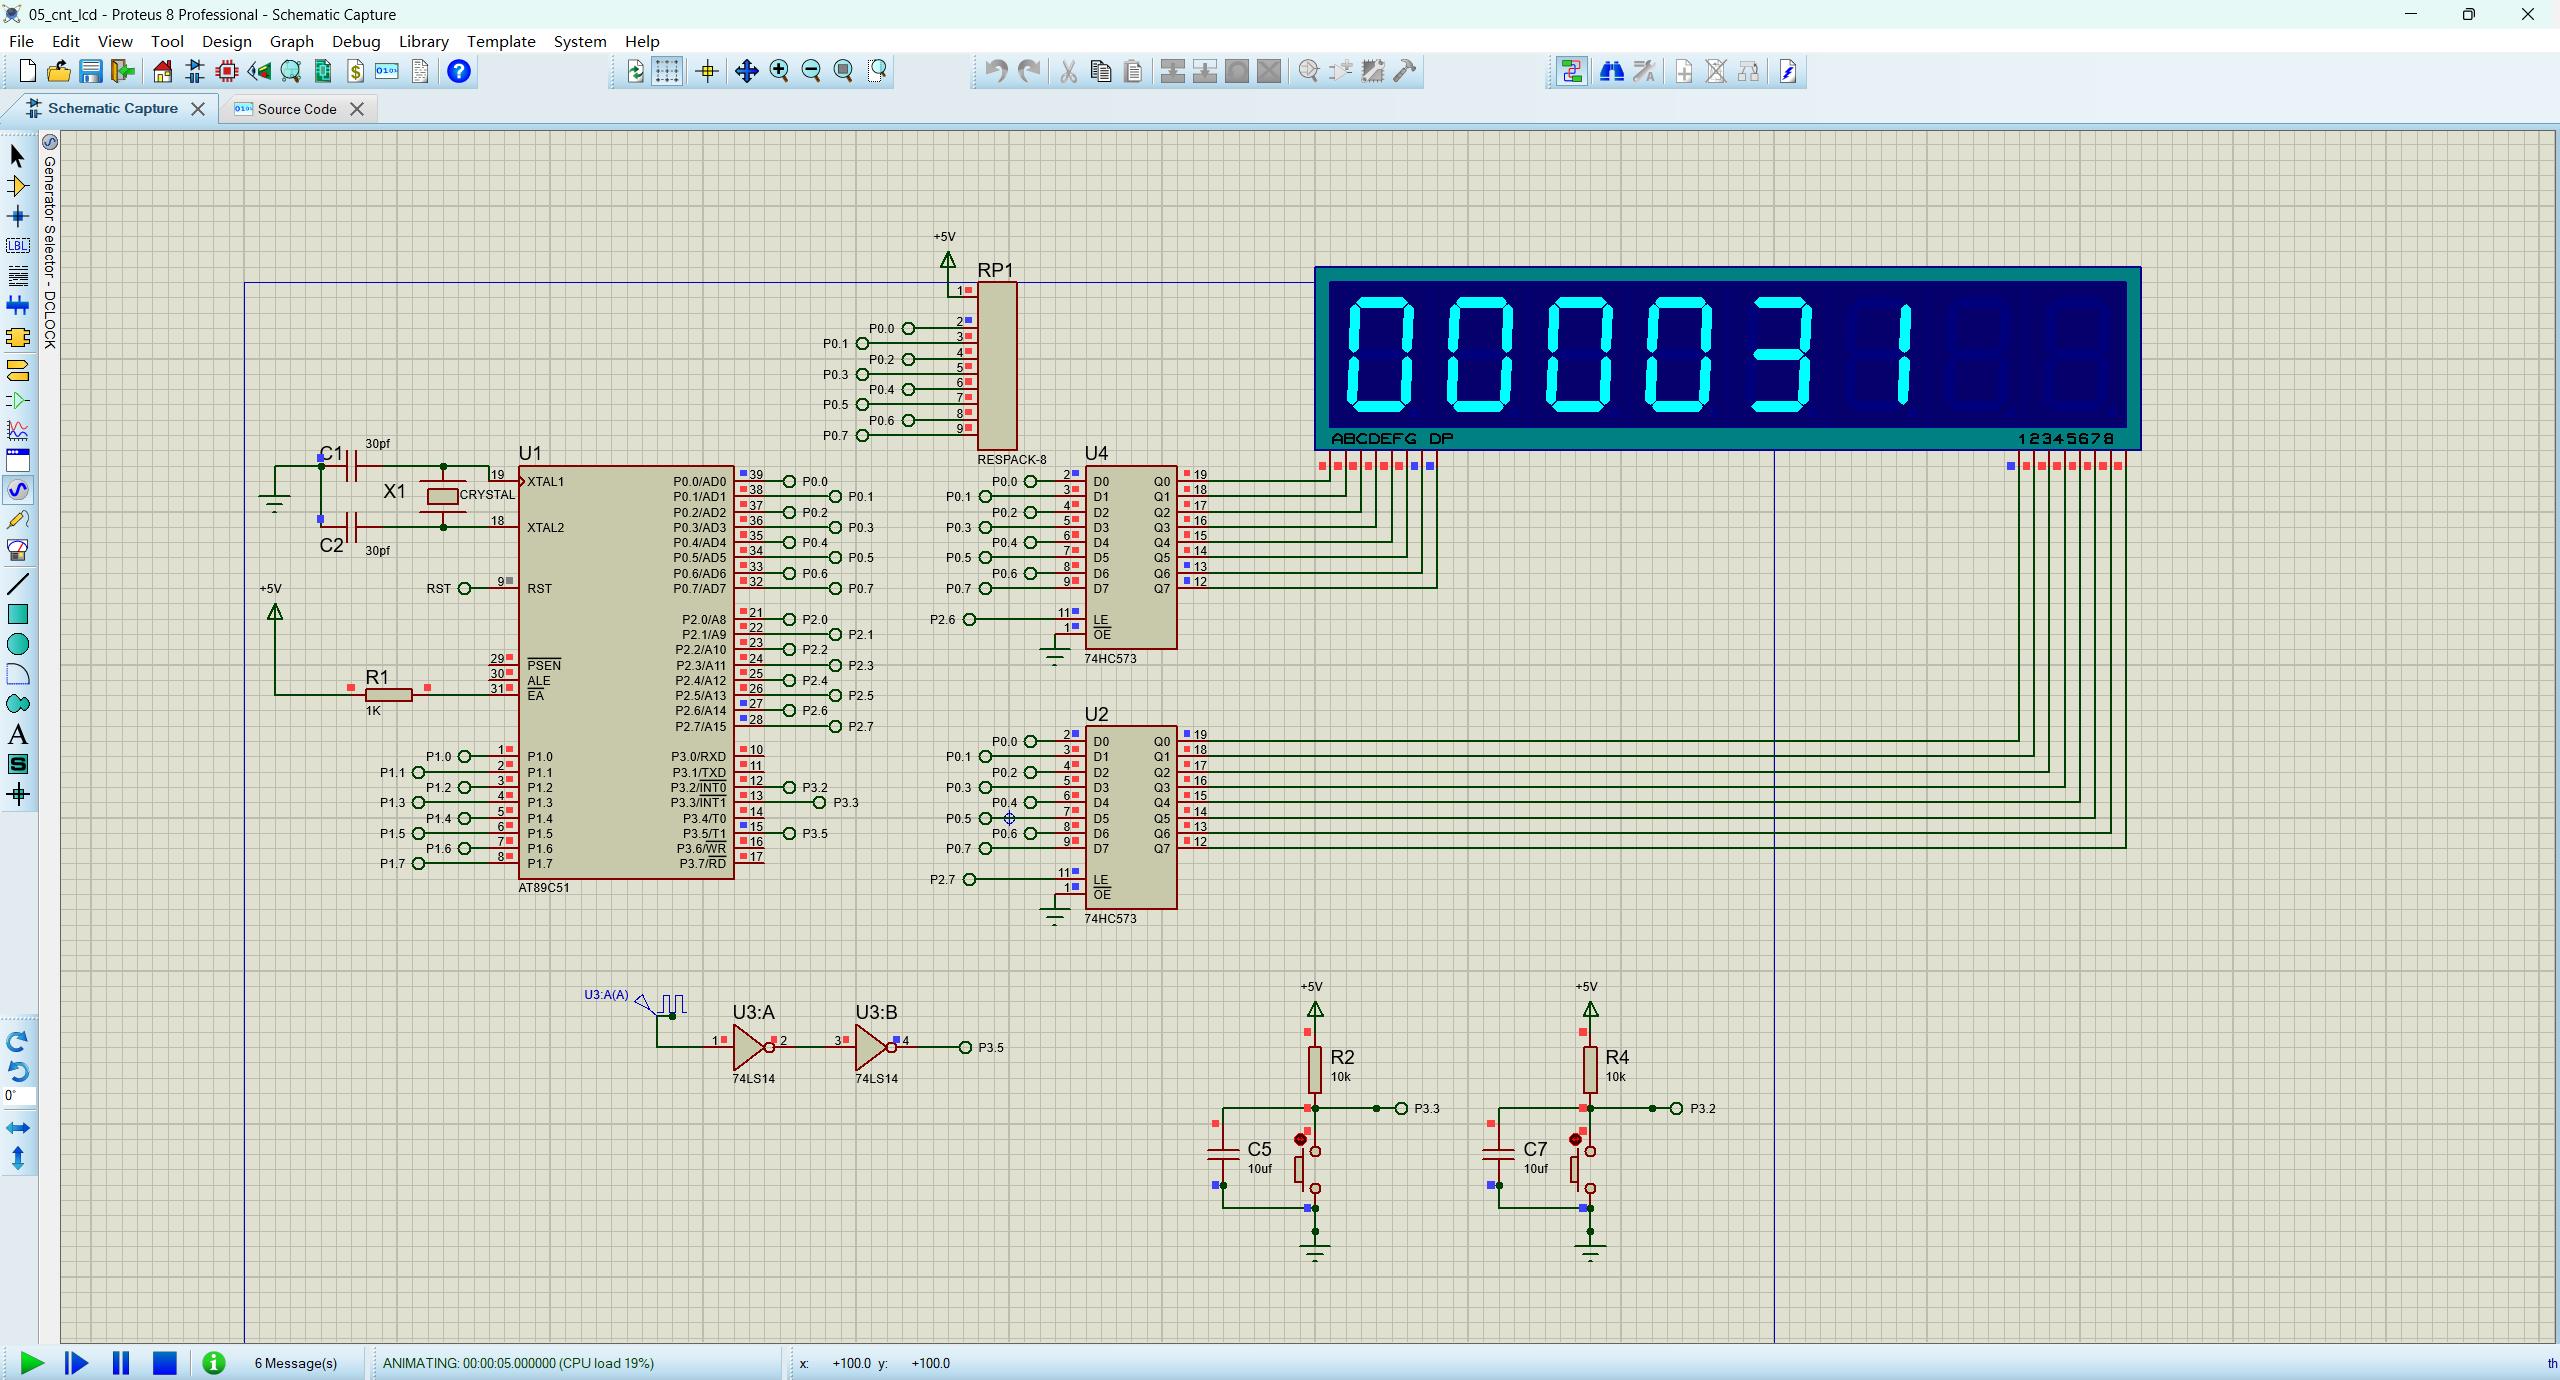
\includegraphics[width=0.94\textwidth]{images/experiment5_key.png}
  \caption{实验五脉冲计数显示 Proteus 关键电路}
\end{figure}

\subsection{调试过程}
\begin{enumerate}
  \item 先验证显示部分，确认系统复位后能够稳定显示 ``000000''。
  \item 检查 P2.6、P2.7 是否分别控制段码锁存器和位码锁存器，防止段码与位码锁存顺序错误。
  \item 单独按下 INT0，观察运行标志是否切换，并确认 TR1 能被启动或停止。
  \item 向 T1 输入低频脉冲，观察显示值是否每来一个脉冲加 1。
  \item 按下 INT1，检查计数是否停止并恢复到 ``000000''。
\end{enumerate}

\subsection{实验现象}
仿真运行后，系统初始显示为 ``000000''。按下 INT0 后，外部脉冲经 74LS14 整形输入 T1，每产生一个有效脉冲，显示值加 1；再次按下 INT0 后，计数保持不变；继续按下 INT0 后，系统在原有数值基础上继续计数。按下 INT1 后，计数立即停止并清零，显示重新变为 ``000000''。

\section{源程序}

\lstinputlisting[style=a51style,caption={05\_cnt\_lcd.A51 完整源代码}]{code/05_cnt_lcd.A51}

\section{实验总结}
本实验完成了基于 AT89C51 的外部脉冲计数显示系统。硬件上，利用两级 74LS14 对外部脉冲进行整形，通过 T1 端实现脉冲计数输入，并沿用 SN74HC573 扩展 P0 口驱动 LED 数码管；软件上，采用 Timer1 方式 2 计数器模式，使每个脉冲产生一次中断，再通过多字节十进制加 1 子程序更新显示缓冲区。通过 INT0 和 INT1 外部中断，实现了启停和清零控制，达到了实验要求。
